\documentclass[addpoints, 10pt]{exam}
\usepackage[utf8]{inputenc}
\usepackage[T1]{fontenc}
\usepackage{amsmath}
\usepackage{amssymb}
\usepackage{systeme}
\usepackage{svg}
\usepackage{pgfplots}
\usepackage{bm}
\usepackage{multicol}
\usepackage{enumitem}
\usepackage{xcolor}
\usepackage{tikz}
\usepackage{float}
\usepackage[margin=2cm]{geometry}
\usepackage[most]{tcolorbox}
\usepackage{tabularx,booktabs}
\newcolumntype{Y}{>{\centering\arraybackslash}X}

\definecolor{gree}{RGB}{101, 191, 127}
\definecolor{gre}{RGB}{7, 135, 44}
\definecolor{crimson}{RGB}{220, 20, 60}
\definecolor{blu}{rgb}{0.34, 0.6, 0.7}
\definecolor{bl}{rgb}{0.34, 0.8, 0.8}
\pgfplotsset{width=10cm,compat=1.9}

\date{}
\renewcommand{\arraystretch}{1.5}

\title{MATH 4.1EL Assignment 1 \\ Number System}
\author{T Yeung}

\newtcolorbox{mycolorbox}[4]{colback=#2!10,enhanced,title=#1,
	attach boxed title to top left={xshift=-4mm},boxrule=0pt,after skip=0.3cm,before skip=0.5cm,right skip=0cm,breakable,fonttitle=\bfseries,toprule=0pt,bottomrule=0pt,rightrule=0pt,leftrule=4pt,arc=0mm,skin=enhancedlast jigsaw,sharp corners,colframe=#3,colbacktitle=#4,boxed title style={
		frame code={ 
			\fill[#4](frame.south west)--(frame.north west)--(frame.north east)--([xshift=3mm]frame.east)--(frame.south east)--cycle;
			\draw[line width=1mm,#4]([xshift=2mm]frame.north east)--([xshift=5mm]frame.east)--([xshift=2mm]frame.south east);
			\draw[line width=1mm,#4]([xshift=5mm]frame.north east)--([xshift=8mm]frame.east)--([xshift=5mm]frame.south east);
			\fill[#2!40](frame.south west)--+(4mm,-2mm)--+(4mm,2mm)--cycle;
		}
	}
}

\newtcolorbox{mycolorbox2}[2]{colback=#2!10,enhanced,title=#1,
	attach boxed title to top left={xshift=-4mm},boxrule=0pt,after skip=0.3cm,before skip=0.5cm,right skip=0cm,breakable,fonttitle=\bfseries,toprule=0pt,bottomrule=0pt,rightrule=0pt,leftrule=4pt,arc=0mm,colframe=#2,colbacktitle=#2, skin=enhancedmiddle  jigsaw
}

\renewcommand{\solutiontitle}{\noindent\textbf{\underline{Solution:}}\par\noindent}
\newenvironment{defin}[1]{\begin{mycolorbox}{Definition: #1}{green}{gree}{gre}}{\end{mycolorbox}}
\newenvironment{thm}[1]{\begin{mycolorbox}{Theorem: #1}{blue}{blu}{bl}}{\end{mycolorbox}}
\newenvironment{note}[1]{\begin{mycolorbox2}{Note: #1}{gray}}{\end{mycolorbox2}}
\newenvironment{mistake}[1]{\begin{mycolorbox2}{Common mistake: #1}{crimson}}{\end{mycolorbox2}}

\newcommand{\tf}[1][{}]{%
\fillin[#1][0.25in]%
}

\begin{document}
\maketitle

\begin{center}
	\fbox{\fbox{\parbox{5.5in}{\centering
				Answer the questions in the spaces provided on the
				question sheets. If you do not know how to answer 
				a certain question, write down where you get stuck.
				Answers can be corrected to 3 significant figures
				if necessary.
	}}}
\end{center}
\vspace{0.1in}
\makebox[\textwidth]{Name, class, class no.:\enspace\hrulefill}
\vspace{0.2in}
\makebox[\textwidth]{Tutor’s name:\enspace\hrulefill}

\section{Natural numbers and Integers}

	\begin{defin}{Natural numbers $\mathbb{N}$}
		Natural numbers contain $1,2,3, \ldots$ but \emph{does not} contain $0$.
	\end{defin}	

	\begin{defin}{Integers $\mathbb{Z}$}
		\textbf{Integers} include positive integers (natural numbers), 0 (zero) and negative integers. \\
		i.e., $\overbrace{\ldots,-3,-2,-1}^{\text{negative integers}}, \overbrace{0}^{\text{zero}}, \overbrace{1, 2, 3,\ldots}^{\text{ positive integers} }$
	\end{defin}	

\begin{questions}
	\fullwidth {
		Determine whether the following statements concerning integers are true. If they are not true, suggest a counterexample.
	}

	\question \tf[T] If we pick any two distinct natural numbers $a$ and $b$, there must be an natural number  $c$ satisfying $a < c < b$.

	\question \tf[T] If we pick any two natural numbers $a$ and $b$, $a+b$ must also be a natural number.

	\question \tf[F] If we pick any two natural numbers $a$ and $b$, $a-b$ must also be a natural number.

	\question \tf[T] If we pick any two natural numbers $a$ and $b$, $a\times b$ must also be a natural number.

	\question \tf[F] If we pick any two natural numbers $a$ and $b$, $\frac{a}{b}$ must also be a natural number.

	\question \tf[T] If we pick any two integers $a$ and $b$, $a+b$ must also be an integer.

	\question \tf[T] If we pick any two integers $a$ and $b$, $a-b$ must also be an integer.

	\question \tf[T] If we pick any two integers $a$ and $b$, $a \times b$ must also be an integer.

	\question \tf[F] If we pick any two integers $a$ and $b$, $\frac{a}{b}$ must also be an integer.

	\newpage 
	\fullwidth{\section{Rational numbers}}
	\fullwidth {
		\begin{defin}{Rational numbers $\mathbb{Q}$}
			A number that can be expressed as a ratio of two integers $i.e., \frac{p}{q}$, where $p$ and $q$ are integers with $q\neq 0$, is called a rational number.
			e.g., $\frac{1}{4}, -1 -\frac{2}{3}, \ldots$
		\end{defin}	
	}

	\fullwidth {
		Determine whether the following statements concerning rational numbers are true. If they are not true, suggest a counterexample.
	}

	\question \tf[T] If we pick any two distinct rational numbers $a$ and $b$, there must be a rational number $c$ satisfying $a < c < b$.

	\question \tf[T] If we pick any two rational numbers $a$ and $b$, $a+b$ must also be a rational number.

	\question \tf[F] If we pick any two rational numbers $a$ and $b$, $a-b$ must also be a rational number.

	\question \tf[T] If we pick any two rational numbers $a$ and $b$, $a \times b$ must also be a rational number.

	\question \tf[F] If we pick any two rational numbers $a$ and $b$, $\frac{a}{b}$ must also be a rational number.

	\fullwidth {
		\begin{mistake}{Dividing by $0$}
			For any number $n$ (belonging to any of the following sets $\mathbb{N}/\mathbb{Z}/\mathbb{Q}/\mathbb{R}/\mathbb{C}$), $\frac{n}{0}$ is \textbf{always undefined}! ($\frac{0}{0}$ is also undefined).
		\end{mistake}
		\subsection{Recurring decimals}
		\begin{defin}{Non-terminating/terminating decimals}
			A \textbf{non-terminating decimals} is a number with a \textbf{non-ending} 
			decimals. For example,
			\begin{itemize}
				\item $\pi = 3.14159265358\ldots$
				\item $\frac{1}{3}=0.33333333333\ldots$
				\item $\frac{1}{7}=0.14285714285\ldots$
				\item $\sqrt{2} = 1.4142135623\ldots$
			\end{itemize}
			On the other hand, a \textbf{terminating decimals} is a number with 
			a decimal part that can be represented with a \textbf{finite} 
			number of digits. For example,
			\begin{itemize}
				\item $\frac{1}{5}=0.2$
				\item $\sqrt{1.21}=1.1$ 
				\item $2.1234$
			\end{itemize}
		\end{defin}
	}

	\question \tf [T] $0.2357$ is a terminating-decimal.

	\question \tf [F] $\pi$ is a terminating-decimal.

	\question \tf [T]	The difference of two terminating decimal must also be a terminating decimal or an integer. 

	\question \tf [F]	The difference of two non-terminating decimal must also be a non-terminating decimal or an integer. 

	\newpage

	\question \tf [F] The solution(s) to $x^2-2=0$ are rational numbers.

	\question Convert $0.12345$ into a fraction. \answerline[2469/20000]

	\fullwidth {
		\begin{defin}{Recurring decimals}
			The notation $0.\overline{12345}$ (or $0.\dot{1}234\dot{5}$) denotes a \textbf{recurring decimal} 
			$0.123451234512345\ldots$ repeating indefinitely. 
			The decimal is \textbf{non-terminating} and \textbf{recurring} 
			(meaning repeating the same sequence of numbers again and again). 
			We can show:
			\begin{align*}
				x  &= 0.\overline{12345} \\
				100000x &= 12345.\overline{12345} \\
				100000x &= 12345 + 0.\overline{12345} \\
				100000x &= 12345 + x \\
				99999x &= 12345 \\
				x &= \tfrac{12345}{99999} \\
				  &= \tfrac{4115}{33333}
			\end{align*}	
		\end{defin}
	}

	\question Write down the number $1.\overline{3}$ up to 6 decimal places. \answerline[0.333333]

	\question Write down the number $12.34\overline{56}$ in 10 significant figures. \answerline[12.34565656]

	\question Write down the number $0.\overline{2}$ as a fraction by using the method illustrated above. 
	\begin{solutionorlines}[5cm]
		\begin{align*}
			y &= 0.\overline{2} \\
			10y &= 2.\overline{2} \\
			9y &= 2 \\
			y &= \tfrac{2}{9}
		\end{align*}	
	\end{solutionorlines}

	\question Write down the number $12.34\overline{56}$ as a fraction by using the method illustrated above.
	\begin{solutionorlines}[5cm]
		\begin{align*}
			y &= 12.34\overline{56} \\
			100y &= 1234.\overline{56} \tag{1} \\
			10000y &= 123456.\overline{56} \tag{2} \\
			\intertext{(2) - (1) { gives }}
			10000y - 100y &= 56 \\
			9900y &= 56 \\
			y &= \frac{56}{9900}
		\end{align*}
	\end{solutionorlines}

	\newpage
		
	\fullwidth {
		\begin{note}{Classification of rational numbers}
			All integers, terminating decimal, and recurring decimals are rational numbers. This is because all of them can be written in $\frac{p}{q}$, where $p$ and $q$ are integers and $q \neq 0$. Check q.19, q.22, q.23 if you feel uncertain about this. \\
			The figure below should help you understand this subject better.
			\begin{figure}[H]
				\centering
				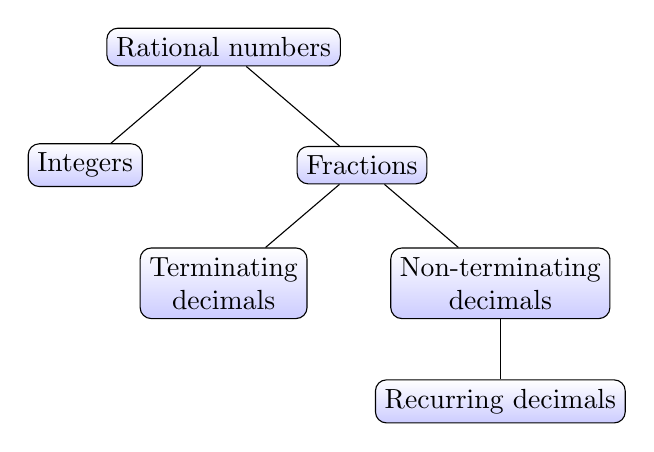
\begin{tikzpicture}[sibling distance=10em,
					every node/.style = {shape=rectangle, rounded corners,
						draw, align=center,
					top color=white, bottom color=blue!20}]]
					\node {Rational numbers}
						child { node {Integers} }
						child { node {Fractions}
							child { node {Terminating \\ decimals} }
							child { node {Non-terminating \\ decimals}
								child { node {Recurring decimals}}
							}
						};
				\end{tikzpicture}
			\end{figure}
		\end{note}
	}

	\begin{comment}
		\begin{mistake}{Not all non-terminating decimals are recurring!}
			It is \emph{true} that all recurring decimals are non-terminating decimals. However, it's \emph{wrong} that all nonterminating decimals are recurring. One counterexample is $\pi$. \\
			This will become clear once we study irrational numbers.
		\end{mistake}
	\end{comment}
	
	\fullwidth {
		Determine whether the following statements concerning irrational numbers are true. 
	}
	\question \tf[T] Given a rational number $n$ is a non-terminating decimal, it must also be a recurring decimal.

	\question \tf[T] All integers are rational numbers.

	\question \tf[T] $0.\overline{314}$ is a rational number.

	\question \tf[F] $\frac{\sqrt{9}}{2}$ is a rational number.

	\question \tf[F] If $\frac{p}{q}$ is rational, then $p$ and $q$ are both rational numbers.
	
	\fullwidth {
		\section{Irrational numbers}
		\begin{defin}{Irrational numbers}
			Irrational numbers are numbers that cannot be expressed as a ratio of two integers (i.e. $\frac{p}{q}$, where $p$ and $q$ are integers with $q \neq 0$) is called an irrational number.
		\end{defin}
		Determine whether the following statements concerning irrational numbers are true. 
		If they are not true, suggest a counterexample.
	}

	\question \tf[T] A real number is either rational or irrational.

	\question \tf[F] If we pick any two irrational numbers $a$ and $b$, $a+b$ must also be a irrational number.

	\question \tf[F] If we pick any two irrational numbers $a$ and $b$, $a-b$ must also be a irrational number.

	\question \tf[F] If we pick any two irrational numbers $a$ and $b$, $a \times b$ must also be a irrational number.

	\question \tf[F] If we pick any two irrational numbers $a$ and $b$, $\frac{a}{b}$ must also be a irrational number.

	\question \tf[T] At least one of $\pi+e$ or $\pi-e$ is irrational.

	\question \tf[F] $\pi=\frac{22}{7}$

	\newpage

	\question \tf[F] $0.\overline{3}$ is irrational.

	\question \tf[F] $1.\overline{2345}$ is irrational.

	\question \tf[F] $0$ is irrational.

	\fullwidth {
		\begin{note}{Classification of irrational numbers}
			All irrational numbers can be expressed as non-terminating and non-recurring decimals.	
		\end{note}
	}

	\question Put tick in the appropriate places in the table. \\
	\smallskip \\
	\begin{tabularx}{0.8\textwidth}{ |c| *{7}{Y|} }
		\cline{2-8}
		\multicolumn{1}{c|}{} &
		\multicolumn{1}{c|}{$4$} &
		\multicolumn{1}{c|}{$0$} &
		\multicolumn{1}{c|}{$-6.2$} &
		\multicolumn{1}{c|}{$\sqrt{15} $} &
		\multicolumn{1}{c|}{$1.\overline{701}$} &
		\multicolumn{1}{c|}{$\frac{\pi}{3}$} &
		\multicolumn{1}{c|}{$-\sqrt{9} $} \\
		\hline
		Natural Number  &  &  &  &  &  &  & \\
		\hline
		Integer    &  &  &  &  &  &  & \\		
		\hline
		Terminating decimal  &  &  &  &  &  &  & \\
		\hline
		Recurring decimal  &  &  &  &  &  &  & \\	
		\hline
		Irrational number &  &  &  &  &  &  & \\
		\hline
	\end{tabularx}
	\fullwidth {
		\section{Real numbers $\mathbb{R}$}
		\begin{defin}{Real numbers $\mathbb{R}$}
			Real numbers include all rational and irrational numbers. Each real number can be represented by a point on a number line.
		\end{defin}

		\begin{note}{Classification of real numbers}
			\begin{figure}[H]
				\centering
				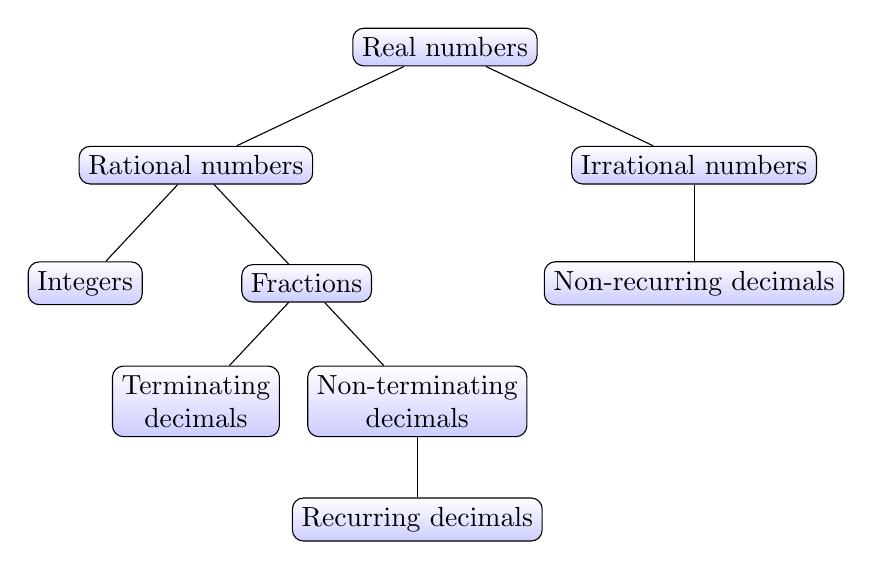
\begin{tikzpicture}[sibling distance=10em,
					level 1/.style ={sibling distance=18em},
					level 2/.style ={sibling distance=8em},
					every node/.style = {shape=rectangle, rounded corners,
						draw, align=center,
					top color=white, bottom color=blue!20}]
					\node {Real numbers}
						child { node{Rational numbers}
							child { node {Integers} }
							child { node {Fractions}
								child { node {Terminating \\ decimals} }
								child { node {Non-terminating \\ decimals}
									child { node {Recurring decimals}}
								}
							}
						}
						child { node{Irrational numbers}
							child {node {Non-recurring decimals}}
						};
				\end{tikzpicture}
			\end{figure}
		\end{note}
	}
	\fullwidth{ Determine whether the following statement is correct }

	\question \tf [F] The solution(s) to $x^2+1=0$ are real numbers.

	\question \tf [F] If $n$ is real number, $n$ must be either integers, terminating decimals or recurring decimals.

	\newpage
	\fullwidth {
	\section{Complex numbers $\mathbb{C}$}
		By adding real numbers with imaginary numbers, 
		we can extend the imaginary numbers further.

		\begin{defin}{Complex numbers $\mathbb{C}$}
			A number that can be written in the form $ a+bi $ is called 
			a \textbf{complex number}, where $a$ and $b$ are real numbers 
			with $ i=\sqrt{-1} $	.
		\end{defin}

		\begin{note}{$\mathbb{N} \subset \mathbb{Z} \subset \mathbb{Q} 
			\subset \mathbb{R} \subset \mathbb{C}$}
			The notation $A \subset B$ means that $B$ contains $A$.
			Note that the set of complex number $(\mathbb{C})$
			contains all numbers.
		\end{note}

		The number $\sqrt{-1}$ is denoted by $i$, which is called the \textbf{imaginary unit}.
		Hence $i^2=-1$ and we say that the equation $x^2+1=0$ has two solutions $x=\pm i$.

		If $N$ is a positive real number, then it is defined that 
		\begin{equation*}
			\sqrt{-N} =\sqrt{N} i
		\end{equation*}
		For example,
		\begin{itemize}
			\item $\sqrt{-2} = \sqrt{2} i$
			\item $\sqrt{-4} = \sqrt{4} i = 2i$
			\item $\sqrt{-9} = \sqrt{9} i = -3i$
		\end{itemize}

		\begin{mistake}{hi} 
			It is incorrect to say that $\sqrt{-9}=\sqrt{-1}\sqrt{9}=3i$ ,
			even though the result is correct.
			This is because $\sqrt{AB} = \sqrt{A} \sqrt{B}$ 
			is only valid for positive real numbers
			$A$ and $B$. \\
			If the theorem extended to negative
			real numbers $A$ and $B$, consider
			\begin{align*}
				\sqrt{9} &= \sqrt{(-3)(-3)} \tag{valid} \\
						 &= \sqrt{-3} \sqrt{-3} \tag{\textbf{\textcolor{red}{invalid!}}} \\
						 &= \sqrt{3} i \sqrt{3} i  \tag{valid}\\
						 &= 3 i^2 \tag{valid}\\
						 &= -3 \tag{valid}
			\end{align*}
			which concludes a contradiction $\sqrt{9} = -3$. 
			Hence, the new theorem cannot be correct. 
			Hence, the rule that $\sqrt{-N} = \sqrt{N} i$ 
			is what we invoked to say $\sqrt{-2} = \sqrt{2} i$, 
			but not $\sqrt{AB} = \sqrt{A} \sqrt{B}$.
		\end{mistake}	
		Express each of the following in the form $bi$, where $b$ is a real number.
	}
	\question $\sqrt{-3}$ \answerline[$\sqrt{3}i$]

	\question $\sqrt{-16}$ \answerline[$4i$]

	\question $-\sqrt{-21}$ \answerline[$-\sqrt{21}i$]

	\question $-\sqrt{-25}$ \answerline[$-5i$]

	\fullwidth {Determine whether the following statement is true.}

	\question \tf[F] It is always true that $\sqrt{A} \sqrt{B} = \sqrt{AB}$ if $A$ and $B$ are real numbers.


	\fullwidth {

		\subsection{Real part and imaginary part}

		\begin{defin}{Real part and imaginary part}
			For a complex number $a+bi$, where $a$ and $b$ are real numbers, 
			$a$ is called the \textbf{real part} and $b$ is called the \textbf{imaginary part}.
		\end{defin}

		\begin{defin}{Purely imaginary number}
			For a complex number $a+bi$, where $a$ and $b$ are real numbers, 
			when $a=0$, the complex number becomes $bi$. We call such
			complex number \textbf{purely imaginary}.
		\end{defin}
		Identify the real part and the imaginary part of each of the following 
		complex numbers. Separate your answer with a semicolon.
	}
	
	\question $1-3i$	\answerline[$1;-3$]
	\question $8-\pi i$	 \answerline[$8;\pi$]
	\question $9$		\answerline[$9;0$]
	\question $\sqrt{-4}-8$	 \answerline[$-8;2$]
	\question $6i-\sqrt{-3} $	\answerline[$0;6-\sqrt{3}$]

	\fullwidth {
		\subsection {Operations of Complex Numbers}
		The usual arithmetic operations with imaginary numbers are similar to 
		that of monomials. You may treat $i$ as a variable first and apply the
		definition of $i = \sqrt{-1}$ later in the process.
	}	
	\newpage
	\fullwidth {
		\begin{note}{Division of complex numbers}
			For complex number of the form $\dfrac{a+bi}{c+di}$,
			you can simplify it by multiplying it by $\dfrac{c-di}{c-di}$
		\end{note}
	}
	\question Simplify the following expressions
	\begin{multicols}{3}
		\begin{enumerate}[label=(\alph*)]
			\item $2i \times 6i$
			\item $(5i+6i)(5i-6i)$
			\item $i^{64}$
			\item $\dfrac{18i^6}{6i^2}$
			\item $\sqrt{-25}-\sqrt{-16}$
			\item $(6+i)^2$
			\item $\dfrac{12+9i}{3}$
			\item $\dfrac{1}{2+2i}$
			\item $\dfrac{1+5i}{2-3i}$
			\item $\dfrac{2-i}{i+3}-\dfrac{i-3}{2+i}$
			\item $i(6+2i)^2$
		\end{enumerate}
	\end{multicols}
	\begin{solutionorlines}[16cm]
	\end{solutionorlines}
	\newpage
	\fullwidth {
		\begin{note}{a+bi=a+bi}
			For real numbers $a, b, c, d$, if $a+bi=c+di$, then $a=c$ and $b=d$
		\end{note}
	}
	\question If $x(3-i)+(y-xi)=-3+4i$, find the values of the real numbers $x$ and $y$.
	\begin{solutionorlines}[5cm]
	\end{solutionorlines}
	\question Draw a tree that relates complex numbers, real numbers, rational numbers, integers, positive integers, zero, and negative integers. Add suitable categories if needed to make your tree complete. Give examples to each category.
	\begin{solutionbox}{10cm}
	\end{solutionbox}
	\newpage
	\question If $2a+3i-2\left( \dfrac{2+bi}{1+i} \right) = (a+1)+4i$, find the values of the real numbers $a$ and $b$.
	\begin{solutionorlines}[5cm]
		
	\end{solutionorlines}

\end{questions}

\end{document}



